\chapter{Architecture \& Modules Integration}
\label{chapter5}

\section{Architecture}

\begin{figure}[H]
  \begin{center}
    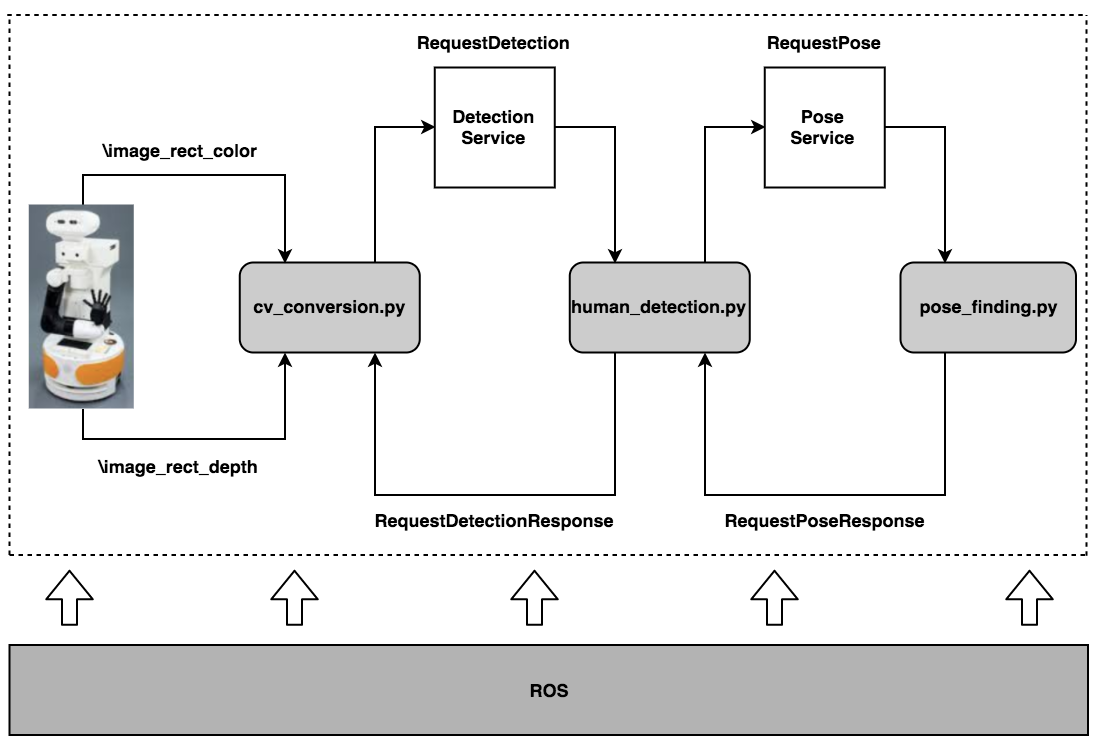
\includegraphics[width=\linewidth]{images/chapter6_architecture.png}
  \end{center}
  \caption{Project's architecture.}
  \label{fig:architecture}
\end{figure}

The final solution has three main components to it:

\begin{enumerate}
	\item The conversion script that converts the \textbf{image\_rect\_color} into an OpenCV format.
    \item The detection script that detects people in the converted image.
    \item The pose script that computes the detection's distance and finds its 3D position in the map.
\end{enumerate}

All of the components do sit on top of the ROS middleware whose utilities include ROS services, standard messages and publish-subscribe communication paradigms among others. Moreover, it is essential to have a ROS master available for the package to work, as this makes available the required topics such as the rectified coloured image and the rectified depth-image. For this project the master node was available through TIAGO's bring-up and its ROS master export in the development machine. 

Finally, ROS services were used for module-intra-communication. Figure \ref{fig:architecture} gives an overview of how the communication happens and in which order between the various components.

\subsection{Communication Logic}

\subsection{Conversion}

The conversion module was implemented via a set of routines called by the main within the same file. This ultimately subscribes to the rectified colour and depth image, converts the former and sends a service request to the detection module, which will respond with a success or failure message (once the whole communication chain is resolved).

\subsection{Detection}

The detection module waits until the service request from the conversion script is received, and upon which it runs the feed-forward process, creates a Detections message and passes this to the next module via a different service request.

\subsection{3D Pose}

Finally the pose module receives the request from the detection one, computes the distance for every detection and its 3D pose in the map. Once done, a set of markers are published to RVIZ along with a custom Poses message with the 3D position for each detection. Lastly a response notifying the success of failure of the process is sent back to the service caller.

\section{Modules Integration}

The original development plan consisted in having separate modules for each task that operates independently of each other, and that would have access to each others computations via the published topics. 

However, this had to be reconsidered when the pose and detection modules had to be integrated. In fact, given that the subscribed depth-image published by TIAGO's interface has a lower publishing rate then the coloured image, a synchronisation problem happened. As the wrong depth ROI\footnote{Region of Interest} was accessed because of the delay, which ultimately consisted in computing the wrong distance and the wrong 3D position.

\subsection{Time Synchroniser}

To solve the synchronisation problem an approximate time synchroniser was used. More precisely the \textbf{ApproximateTimeSynchronizer} routine made available by the message\_filters library. This allows the subscription to multiple topics whose callback function is called only when the timestamps differences are within a certain threshold.

Therefore, two separate subscriptions called \textbf{rgb\_sub} and \textbf{depth\_sub} were made respectively to the raw rectified image and the rectified depth-image topics in the conversion script. The two are then chained together using the time synchronizer with a threshold error of at most 0.5 seconds, as shown below. Of course, the bigger the threshold, the greater the delay, hence a good empirical value had to be found. The synchronisation is then binded to a callback function called \textbf{processSubscriptions} using the \textbf{registerCallback} routine, also made available by the message\_filters library as follows.

\begin{lstlisting}
import message_filters as mf
ats = mf.ApproximateTimeSynchronizer([rgb_sub, depth_sub], slop=0.5)
ats.registerCallback(processSubscriptions)
\end{lstlisting}

\subsection{ROS Services}

Two choices were available for the module-intra-communication, either using standard publish-subscribe communication or an RPC\footnote{Remote Procedure Call} based style via services. 

The original idea was to use the former type of communication, as it would allow a more flexible and modular usage of the package. Given that if a user only wants to use a specific component, only the required module would have to be executed. However, due to the RGB-depth synchronisation problem, and the fact that the subscriptions are both made in one place (the conversion script) and not in their relative module as originally planned (so rgb\_sub in the conversion module and depth\_sub in the pose module) the latter type of communication via ROS services was preferred for an easier message exchange. In fact, via a service mean, the collected ROS messages at subscription time can be passed forward to the server nodes with simple \textbf{srv} files rather then having to publish them all over again.

A \textbf{srv} folder was therefore created in the same path as the msg folder at the root of the catkin package, in which two services are defined. A detection one called \textbf{RequestDetection.srv} that requests the feed-forward process to the detection module and that has as a client the conversion component and as the server the detection one. A pose service named \textbf{RequestPose.srv} is also declared, which requests the actual distance and 3D pose computation, and whose client and server are respectively the detection and pose modules. The two service declarations for the RequestDetection.srv(left) and the RequestPose.srv(right) are as follows:

\begin{multicols}{2}
  \begin{itemize}
    \item sensor\_msgs/Image depth
    \item - - -
    \item string res
  \end{itemize}

  \columnbreak

  \begin{itemize}
    \item Detections detections
    \item sensor\_msgs/Image depth
    \item - - -
    \item string res
  \end{itemize}
\end{multicols}

A typical service message is made of a request and response field declaration separated by a dotted line. 

The detection's service request, sent by the conversion module, has only the synchronised depth-image as its only field, as the RGB image is stored in the disk. The response expected by the service is a string determining either the success of failure of the service, which is then printed to the console for the user to keep track of the process.

Similarly the pose service request expects as input the detections computed by the neural network as a Detections message, as well as the depth-image originally retrieved during the conversion process at the beginning of the chain. The response expected is again a string suggesting the failure or success of the process.

The service requests are blocking, which means that the module is idled as it waits for the server to come up or the response message to be received, which is something to improve upon in the future.


